\documentclass[a4paper,10pt]{article}

\usepackage{xcolor}
\usepackage{titlesec}
\usepackage{graphicx}
\usepackage{float}
\usepackage{caption}
\usepackage[margin=1.5cm]{geometry}
\usepackage{fancyhdr}
\usepackage{pdfpages}


%\title{Abdelrahman's Document}
%\author{Torpedo}
%\date{March 9, 2024}

\renewcommand{\thesection}{\Alph{section}}
\renewcommand{\thesubsection}{\arabic{subsection}}
\setlength{\parindent}{0pt}
\setlength{\parskip}{0pt}

\definecolor{Red}{RGB}{240, 20, 20}
\definecolor{lightRed}{RGB}{180, 20, 20}
\titleformat{\section}{\color{Red}\normalfont\Large\bfseries}{\thesection}{1em}{\vspace{-\baselineskip}}
\titleformat{\subsection}{\color{lightRed}\normalfont\large\bfseries}{\thesubsection}{1em}{}

\pagestyle{fancy}
\fancyhf{}

\begin{document}
	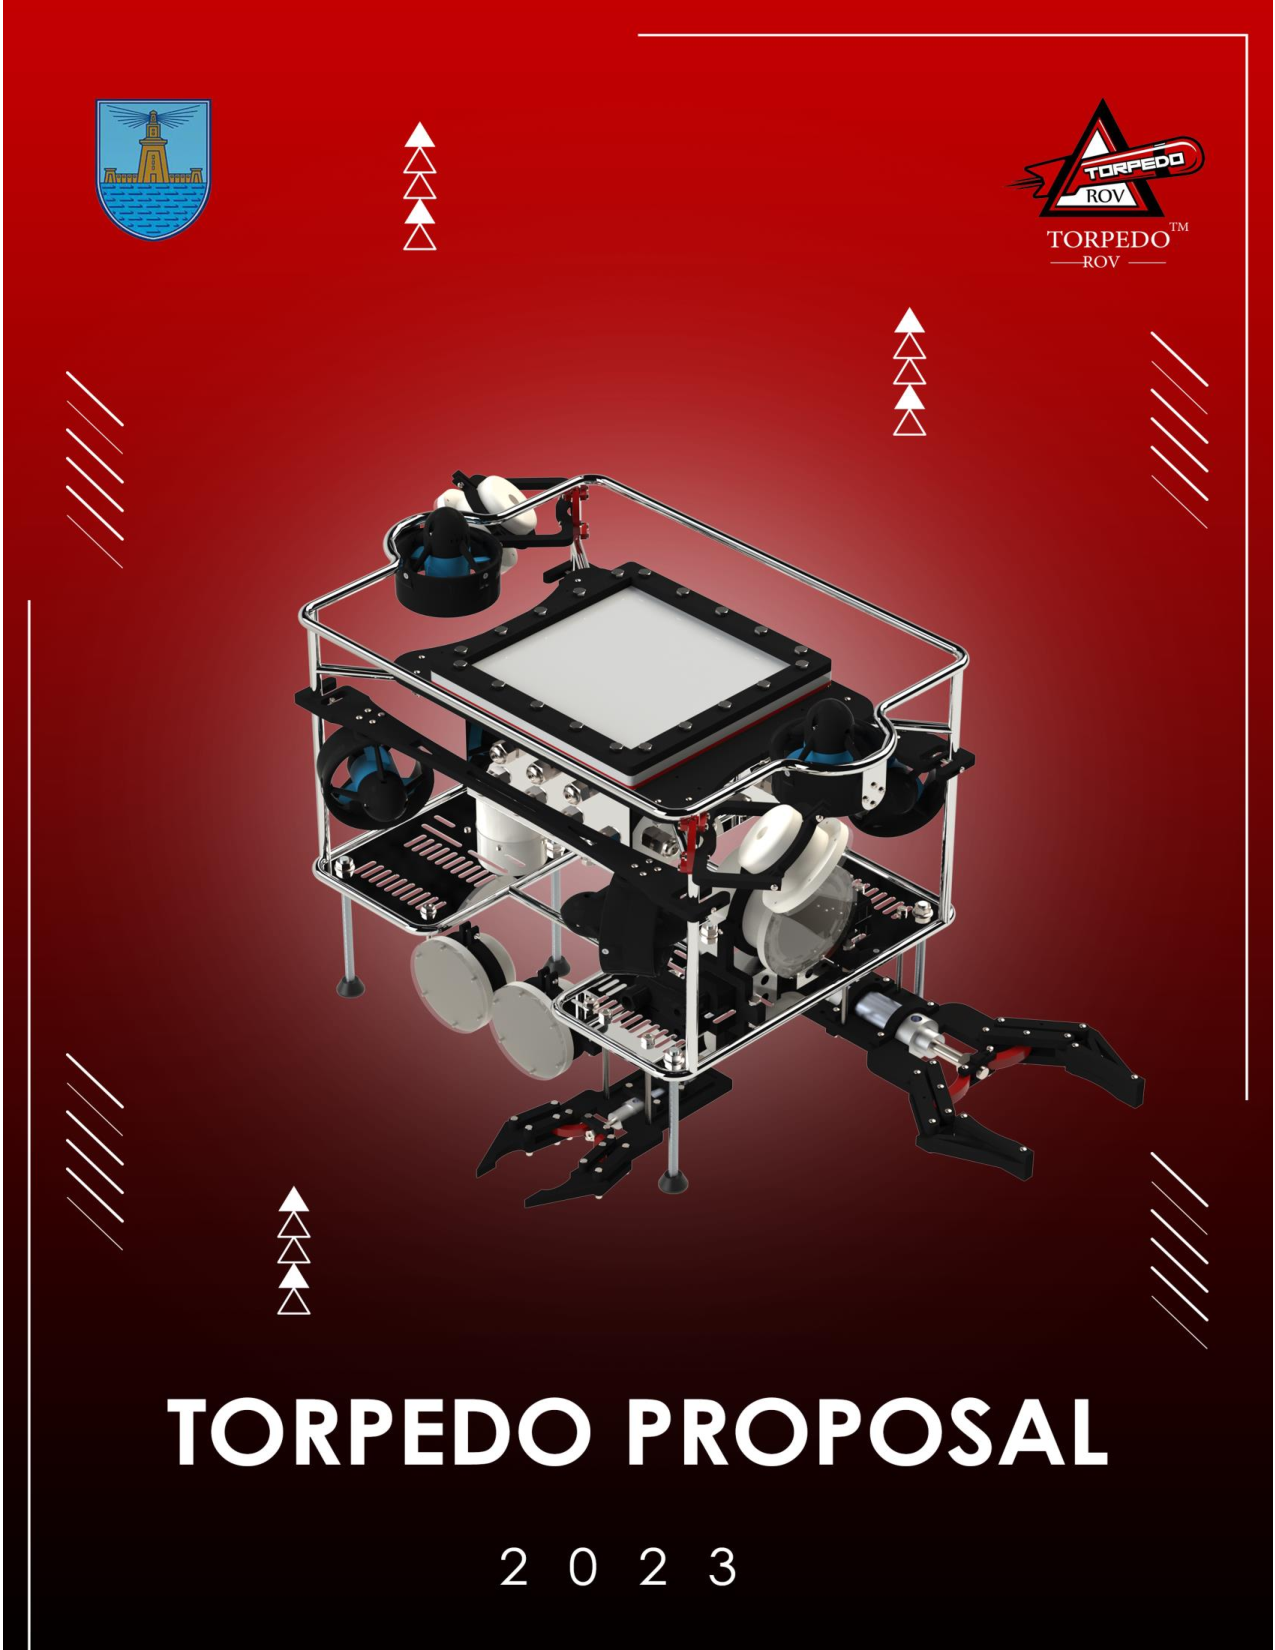
\includepdf[page=1,fitpaper]{Cover_Page}
	\tableofcontents
	\fancyhf{}
	\renewcommand{\headrulewidth}{0pt}
	\setlength{\headsep}{1.5cm}
	\fancyhead[L]{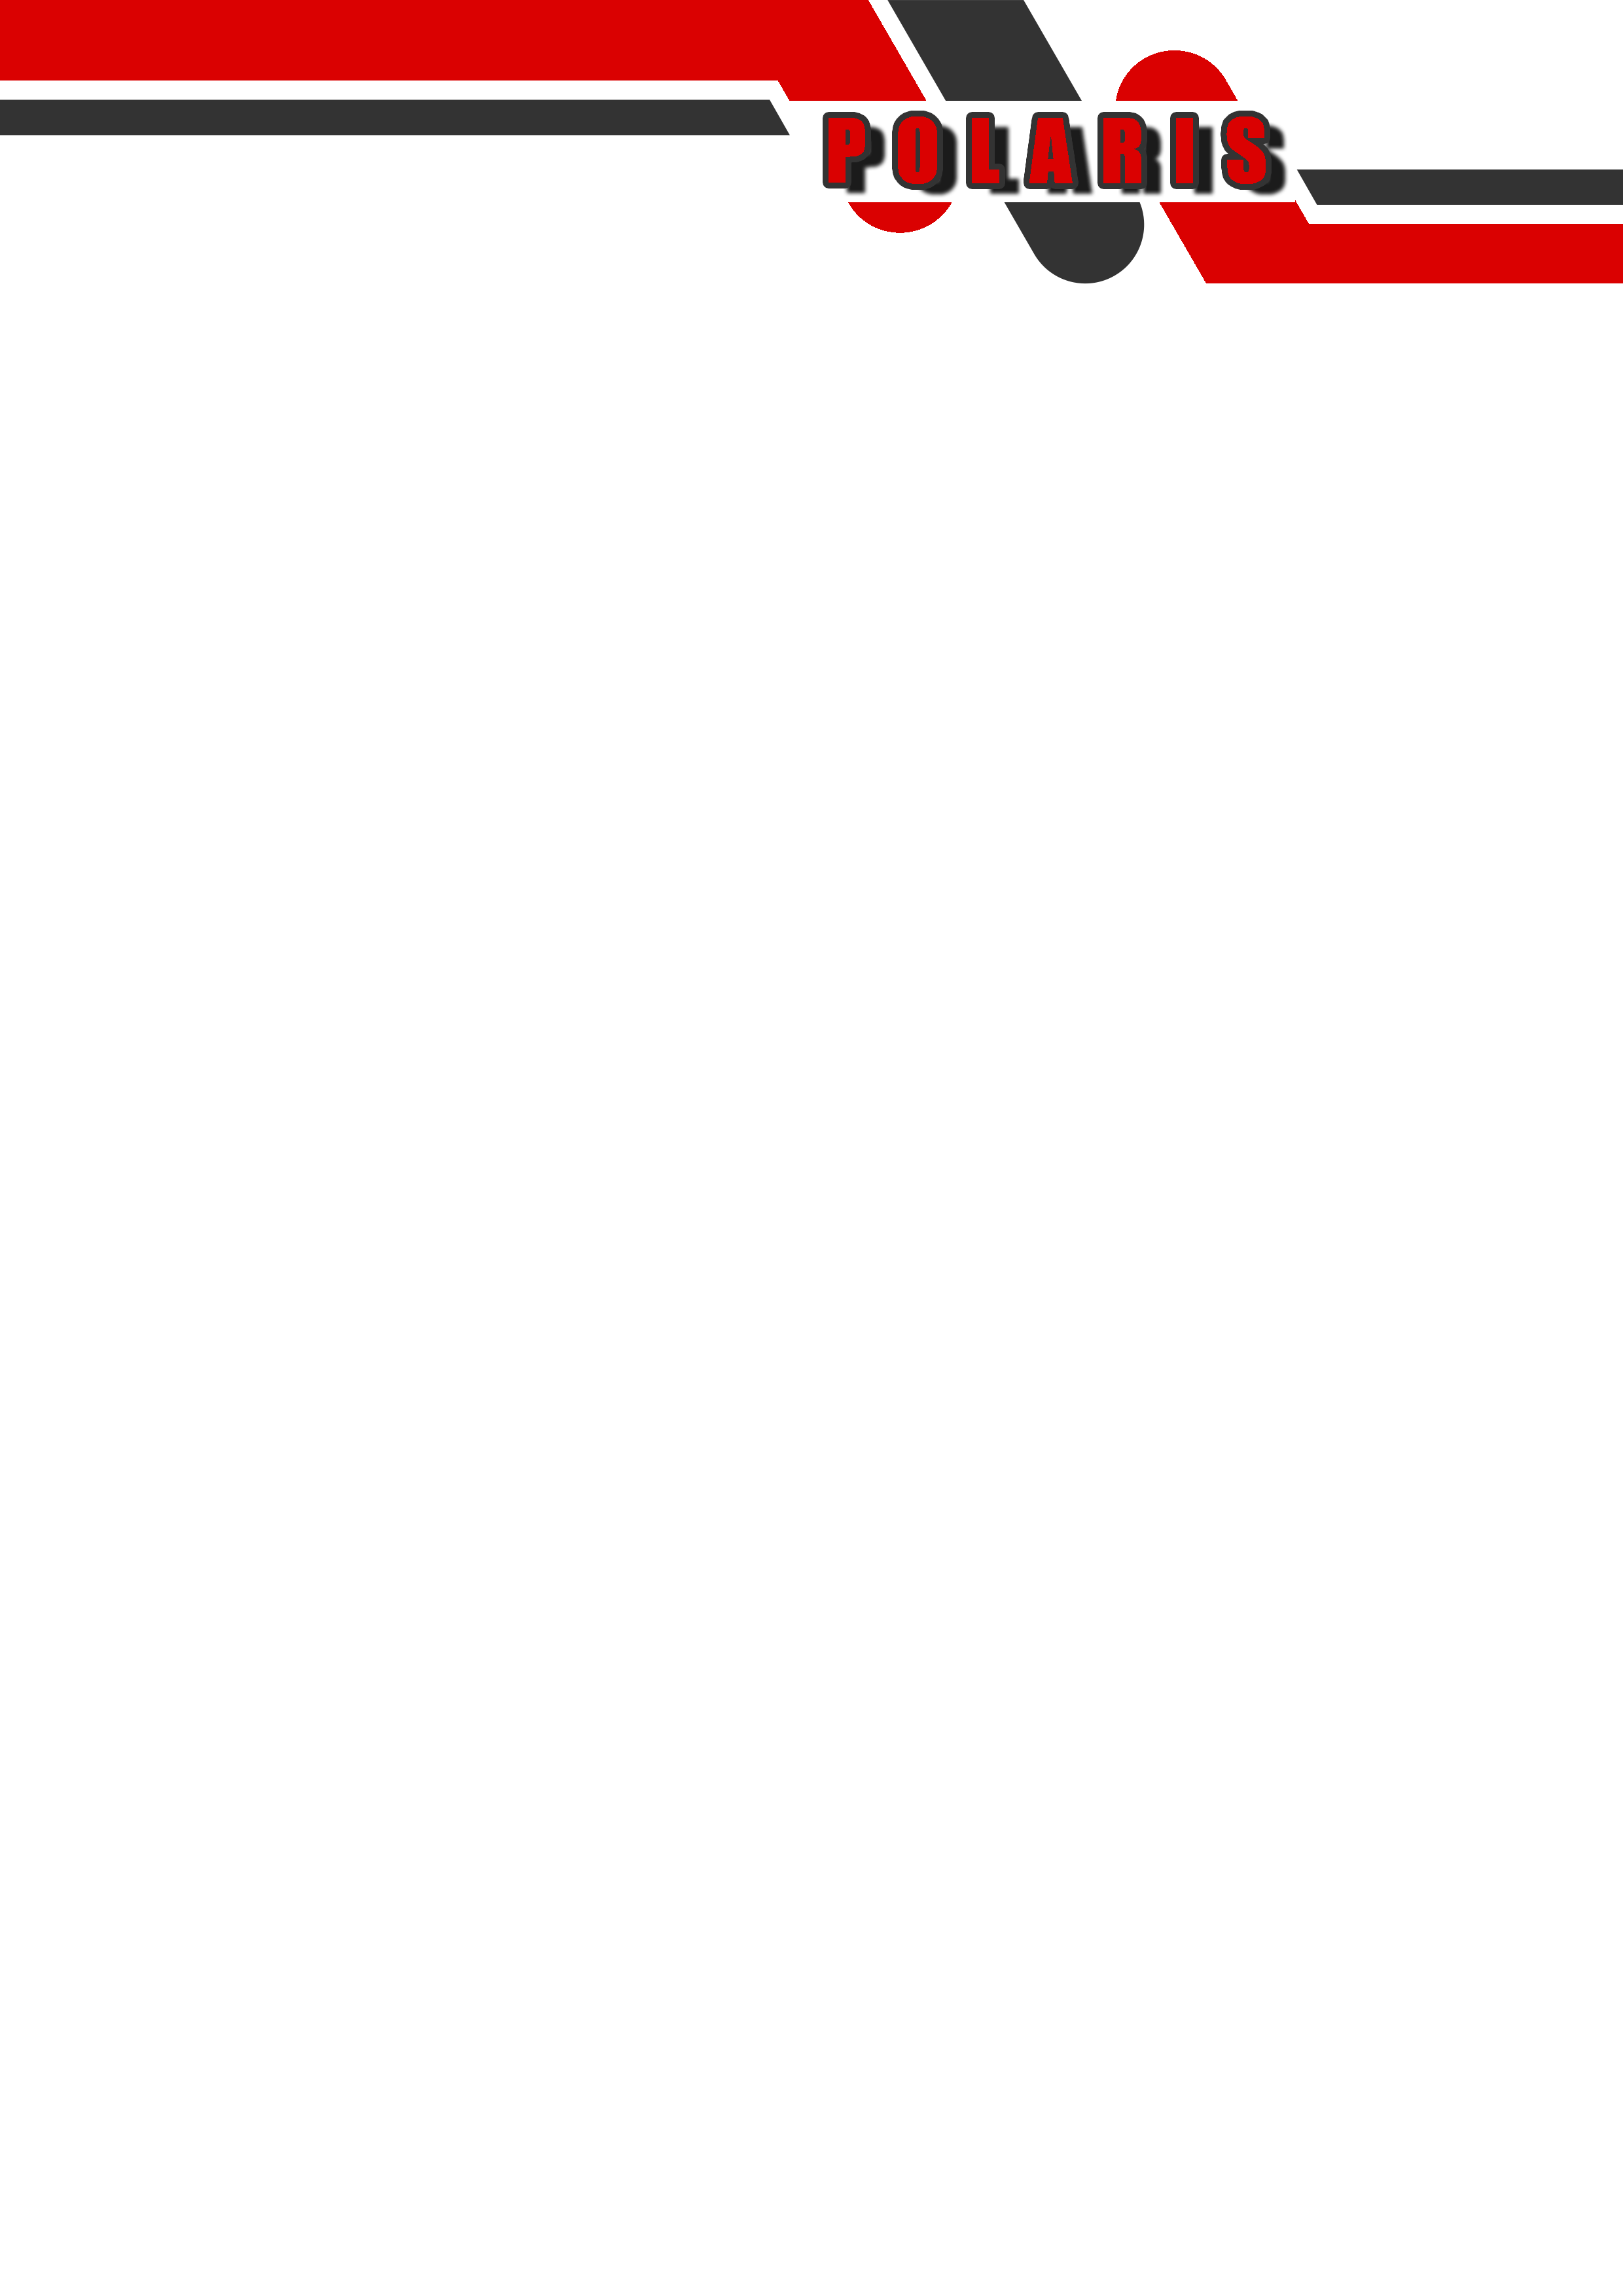
\includegraphics[width=\textwidth, height = .45\textheight]{header}} % WHY L? 
	\fancyfoot{} 
	\fancyfoot[C]{\thepage}
	\newpage
	%\maketitle
	\setcounter{section}{3}
	\section{Software}
	\setcounter{subsection}{0}
	\begin{figure}[H]
		\begin{minipage}{0.6\textwidth}
			\subsection{Thrusters Vector Algorithm:}
			One problem we faced with our previous ROV’s was heavily
			relying on basic motion directions (forward/backward/lateral left/right)
			along with rotational motion on x, y, and z axes. This made the ROV’s 
			diagonal motion hard and slow. This year, with the help of our R\&D
			team, we found the solution to this problem in Jerzy Garus’s paper
			which introduces a vector algorithm which enables us to move the
			ROV in any direction.
		\end{minipage}
		\hfill
		\begin{minipage}{0.35\textwidth}
			\centering
			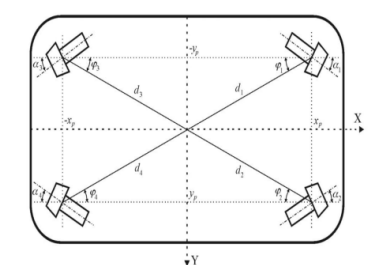
\includegraphics[width=\textwidth]{vector_algorithm}
			\captionof{figure}{Polaris Horizontal Motors Configuration}
		\end{minipage}
	\end{figure}
	\subsection{Thrusters Speed}
		After getting the wanted speed from the pilot, this data will be transmitted to the motors board
		to be applied to the thrusters in the right order to enable Polaris move in a specific direction.  
		
		But assigning these speeds to the thrusters as they are, if the change in speed is large enough
		especially if the motors are in sleep mode before setting the speed for them, may lead to a high
		current draw, which may lead to the destruction of other components or affect the paths of the
		board itself.
		
		At that moment comes the role of “soft start”, which is to prevent the high current draw or
		malfunctioning of thrusters that could happen when a sudden change of the thrusters’ speed
		occurs. We implemented our own software-based soft starter, by gradually ramping up the
		speed supplied to the thrusters.
	
	\section{Communication}
	\renewcommand{\thesubsection}{\Roman{subsection}}
	\begin{figure}[H]
		\begin{minipage}{0.65\textwidth}
			\subsection{Top side:}	
			As for the communication between the TCU and Polaris, Ethernet UDP “User 
			Datagram Protocol” was used. The communication is full duplex; hence 
			Polaris can send and receive data simultaneously. ENC28J60 Ethernet 
			controller was chosen to serve as an ethernet network interface for the used 
			microcontrollers since they are equipped with SPI “Serial Peripheral 
			Interface”. On top of that, the “UIPEthernet” library was used to control the 
			Ethernet modules
		\end{minipage}
		\hfill
		\begin{minipage}{0.3\textwidth} 
			\centering
			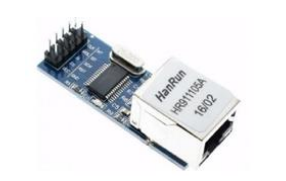
\includegraphics[width=\textwidth]{ethernet_module}
			\captionof{figure}{Ethernet Module}
		\end{minipage}
	\end{figure}
	\subsection{Underwater side}
		This year, we decided to use an ESP32 microcontroller instead of using three Arduino Nano. 
		This reduced the error due to communication between the three Arduino Nanos. The ESP32 
		offered several advantages over the Arduino such as its higher processing power, its dual core 
		architecture which allowed us to multitask and its built-in Wi-Fi which allowed us to upload 
		different codes on Polaris’ ESP32 wirelessly.
	
	\section{Vision System}
	\begin{figure}[H]
		\begin{minipage}{0.7\textwidth}
			\subsection*{Camera Control}
			We have used a camera module that is made to operate and receive feeds 
			from the cameras on the ROV. It can capture and process video feeds from 
			various types of cameras. Moreover, it can be configured to work with either 
			an external or local camera, depending on the specific requirements of the 
			task. The module also provides advanced features for managing video 
			streams, such as handling lost connections and automatically 
			reconnecting to the camera when required
		\end{minipage}
		\hfill
		\begin{minipage}{0.2\textwidth}
			\centering
			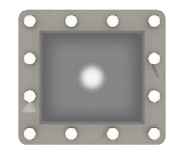
\includegraphics[width=\textwidth]{main_camera}
			\captionof{figure}{Polaris Horizontal Motors Configuration}
		\end{minipage}
		
		
		
	\end{figure}
	
	
	
\end{document}